\chapter{Ionaire en moleculaire vaste stoffen oplossen}\label{ch:g11:dissolution}

Een snufje zout dat je door water roert, verdwijnt in een paar seconden;
hetzelfde snufje door slaolie geroerd, blijft onveranderd op de bodem van
het glas liggen, zolang je er ook naar kijkt. Een vette pan die je onder
de kraan afspoelt, blijft vet; één druppel afwasmiddel, en het vet laat
los. Wat bepaalt of een stof in een vloeistof \omterm{def:g2:mixing-and-dissolving:dissolve}{oplost}? Het antwoord zit
in de \omterm{def:g11:polarity-and-cohesion:polar-bond}{partiële ladingen} en de krachten tussen deeltjes uit het vorige
hoofdstuk.

\begin{recall}
\omterm{def:g6:solutions-and-solubility:solubility}{Oplosbaarheid}; \omterm{def:g6:solutions-and-solubility:miscible}{mengbare} en \omterm{def:g6:solutions-and-solubility:miscible}{niet-mengbare} vloeistoffen
(\cref{ch:g6:solutions-and-solubility}). Een \omterm{def:g9:ions:ionic-compound}{ionverbinding} bestaat uit
\omterm{def:g9:ions:ion}{kationen} en \omterm{def:g9:ions:ion}{anionen} in verhoudingen die haar neutraal maken
(\cref{ch:g9:ions}). Polaire en \omterm{def:g11:polarity-and-cohesion:polar-molecule}{apolaire moleculen}, \omterm{def:g11:polarity-and-cohesion:hydrogen-bond}{waterstofbruggen},
\omterm{def:g11:polarity-and-cohesion:van-der-waals}{vanderwaalsbindingen} (\cref{ch:g11:polarity-and-cohesion}).
\omterm{def:g10:chemical-species:extraction}{Vloeistof-vloeistofextractie} (\cref{ch:g10:chemical-species}). \omterm{def:g10:concentration-and-dilution:molar-concentration}{Molaire
concentratie} (\cref{ch:g10:concentration-and-dilution}).
\end{recall}

\section{Een ionaire vaste stof oplossen}

In een kristal natriumchloride is elk natriumion \ce{Na+} omringd door
\omterm{def:g9:ions:ion}{chloride-ionen} \ce{Cl-} en elk \omterm{def:g9:ions:ion}{chloride-ion} door natriumionen, allemaal
bijeengehouden door de aantrekking tussen tegengestelde ladingen.
Watermoleculen, die polair zijn, worden door deze ladingen aangetrokken:
hun zuurstofkant ($\delta^-$) draait naar de \omterm{def:g9:ions:ion}{kationen}, hun waterstofkant
($\delta^+$) naar de \omterm{def:g9:ions:ion}{anionen}.

\begin{definition}[Dissociatie]\label{def:g11:dissolution:dissociation}
De \emph{dissociatie}\index{dissociatie} van een ionaire vaste stof in een
\omterm{def:g6:solutions-and-solubility:solute}{oplosmiddel} is het van elkaar loskomen van haar \omterm{def:g9:ions:ion}{ionen}: ze verlaten het
kristal en verspreiden zich in de oplossing.
\end{definition}

\begin{definition}[Solvatatie, hydratatie]\label{def:g11:dissolution:solvation}
De \emph{solvatatie}\index{solvatatie} van een opgelost deeltje is het
omringd worden door \omterm{def:g7:atoms-and-molecules:molecule}{moleculen} van het \omterm{def:g6:solutions-and-solubility:solute}{oplosmiddel}, die er door
aantrekking aan vastgehouden worden; in water heet dat
\emph{hydratatie}\index{hydratatie}. Het symbool (aq) na een formule
betekent ``gehydrateerd''.
\end{definition}

\begin{proposition}[Drie stadia van oplossen]\label{prop:g11:dissolution:stages}
Een ionaire vaste stof lost in water op in drie stadia die tegelijk
gebeuren: de \omterm{def:g9:ions:ion}{ionen} worden uit het kristal getrokken (\omterm{def:g11:dissolution:dissociation}{dissociatie}),
omringd door watermoleculen (\omterm{def:g11:dissolution:solvation}{hydratatie}), en over de hele oplossing
verspreid (dispersie). Voor natriumchloride:
\[
  \ce{NaCl(s) -> Na+(aq) + Cl-(aq)} .
\]
\end{proposition}

\begin{proof}
Aangenomen: de aantrekkingen tussen de \omterm{def:g9:ions:ion}{ionen} en de polaire watermoleculen
zijn samen sterk genoeg om die tussen de \omterm{def:g9:ions:ion}{ionen} van het kristal te
vervangen.
\end{proof}

\begin{omfigure}
\begin{tikzpicture}[font=\small]
  % the crystal edge: alternating ions
  \foreach \i in {0,1,2,3,4} \foreach \j in {0,1,2,3} {
    \pgfmathtruncatemacro\k{mod(\i+\j,2)}
    \ifnum\k=0
      \node[om atom, ball color=green!60!black, minimum size=6.4mm] at (0.8*\i,0.8*\j) {};
    \else
      \node[om atom, ball color=violet!70, minimum size=4.0mm] at (0.8*\i,0.8*\j) {};
    \fi
  }
  % a hydrated Na+ that has left: O towards the ion
  \begin{scope}[shift={(5.6,1.8)}]
    \node[om atom, ball color=violet!70, minimum size=4.0mm] (na) at (0,0) {};
    \node[font=\footnotesize] at (0,0) {};
    \foreach \a in {0,90,180,270} {
      \node[aO, minimum size=4.6mm] (o\a) at (\a:0.62) {};
      \node[aH, minimum size=3.2mm] (ha\a) at ($(\a:0.62)+(\a+52:0.42)$) {};
      \node[aH, minimum size=3.2mm] (hb\a) at ($(\a:0.62)+(\a-52:0.42)$) {};
      \begin{scope}[on background layer]
        \draw[bond, line width=1.2pt] (o\a.center) -- (ha\a.center);
        \draw[bond, line width=1.2pt] (o\a.center) -- (hb\a.center);
      \end{scope}
    }
    \node[anchor=north] at (0,-1.35) {\ce{Na+(aq)}};
  \end{scope}
  % a hydrated Cl- that has left: H towards the ion
  \begin{scope}[shift={(8.6,1.4)}]
    \node[om atom, ball color=green!60!black, minimum size=6.4mm] at (0,0) {};
    \foreach \a in {45,135,225,315} {
      \node[aH, minimum size=3.2mm] (h\a) at (\a:0.62) {};
      \node[aO, minimum size=4.6mm] (o\a) at (\a:1.0) {};
      \node[aH, minimum size=3.2mm] (k\a) at ($(\a:1.0)+(\a+75:0.42)$) {};
      \begin{scope}[on background layer]
        \draw[bond, line width=1.2pt] (o\a.center) -- (h\a.center);
        \draw[bond, line width=1.2pt] (o\a.center) -- (k\a.center);
      \end{scope}
    }
    \node[anchor=north] at (0,-1.45) {\ce{Cl-(aq)}};
  \end{scope}
  \node[anchor=north, align=center] at (1.6,-0.45) {het kristal\\
    (\ce{Na+} klein, \ce{Cl-} groot)};
\end{tikzpicture}

{\small Natriumchloride \omterm{def:g2:mixing-and-dissolving:dissolve}{lost op}. Een natriumion en een \omterm{def:g9:ions:ion}{chloride-ion} hebben
het kristal verlaten; elk is gehydrateerd. Rond het \omterm{def:g9:ions:ion}{kation} draaien de
watermoleculen hun zuurstofatomen (rood, $\delta^-$) naar binnen, rond het
\omterm{def:g9:ions:ion}{anion} hun waterstofatomen (wit, $\delta^+$).}
\end{omfigure}

\section{Concentraties van de ionen}

\begin{method}[Concentratie van elk ion]\label{met:g11:dissolution:ions}
\begin{enumerate}
  \item Schrijf de oplosvergelijking op, kloppend in \omterm{def:g7:atoms-and-molecules:atom}{atomen} en in lading:
        voor calciumchloride, \ce{CaCl2(s) -> Ca^{2+}(aq) + 2Cl-(aq)}.
  \item Bereken de hoeveelheid $n$ opgeloste vaste stof, en de
        concentratie $c = n / V$ van de oplossing aan \omterm{def:g6:solutions-and-solubility:solute}{opgeloste stof}.
  \item Elk \omterm{def:g9:ions:ion}{ion} heeft de concentratie $c$ vermenigvuldigd met zijn
        \omterm{def:g8:balanced-equations:coefficient}{coëfficiënt} in de vergelijking: hier $[\ce{Ca^{2+}}] = c$ en
        $[\ce{Cl-}] = 2c$.
\end{enumerate}
De vierkante haken $[\ldots]$ geven de \omterm{def:g10:concentration-and-dilution:molar-concentration}{molaire concentratie} van een
\omterm{def:g6:solutions-and-solubility:solute}{opgeloste stof} aan.
\end{method}

\begin{example}[Calciumchloride]\label{ex:g11:dissolution:cacl2}
% ledger: aw:Ca, aw:Cl
\qty{5.55}{g} calciumchloride ($M = \qty{111.1}{g/mol}$) opgelost tot
\qty{500.0}{mL} oplossing: $n = \qty{0.0500}{mol}$,
$c = \qty{0.100}{mol/L}$, dus $[\ce{Ca^{2+}}] = \qty{0.100}{mol/L}$ en
$[\ce{Cl-}] = \qty{0.200}{mol/L}$. De oplossing is neutraal: $2 \times
0.100$ positieve lading per liter tegenover $1 \times 0.200$ negatieve.
\end{example}

\section{Polariteit en oplosbaarheid}

\begin{proposition}[Soort zoekt soort]\label{prop:g11:dissolution:like}
Een polair \omterm{def:g6:solutions-and-solubility:solute}{oplosmiddel}, zoals water, lost ionaire vaste stoffen en
polaire stoffen op, vooral die welke er \omterm{def:g11:polarity-and-cohesion:hydrogen-bond}{waterstofbruggen} mee kunnen
vormen; een apolair \omterm{def:g6:solutions-and-solubility:solute}{oplosmiddel}, zoals cyclohexaan of een plantaardige
olie, lost apolaire stoffen op. Ionaire vaste stoffen lossen heel weinig
op in apolaire \omterm{def:g6:solutions-and-solubility:solute}{oplosmiddelen}, en apolaire stoffen heel weinig in water.
\end{proposition}

\begin{proof}
Aangenomen: een stof lost goed op als de aantrekkingen die ze met het
\omterm{def:g6:solutions-and-solubility:solute}{oplosmiddel} kan vormen minstens zo sterk zijn als die welke ze verbreekt,
tussen haar eigen deeltjes en tussen de \omterm{def:g7:atoms-and-molecules:molecule}{moleculen} van het \omterm{def:g6:solutions-and-solubility:solute}{oplosmiddel}.
\end{proof}

\begin{example}[Drie gevallen]\label{ex:g11:dissolution:cases}
% ledger: sol:I2-water, sol:I2-heptane
Ethanol \omterm{def:g2:mixing-and-dissolving:mix}{mengt} in alle verhoudingen met water: zijn \ce{O-H}-groep vormt
\omterm{def:g11:polarity-and-cohesion:hydrogen-bond}{waterstofbruggen} met water. Zout \omterm{def:g2:mixing-and-dissolving:dissolve}{lost op} in water, maar niet in olie.
Jood, \ce{I2}, een \omterm{def:g11:polarity-and-cohesion:polar-molecule}{apolair molecuul}, lost slecht op in water (ongeveer
\qty{0.3}{g/L}, een bruine oplossing) maar goed in apolaire
\omterm{def:g6:solutions-and-solubility:solute}{oplosmiddelen} (\qty{17}{g} per kilogram heptaan, een violette oplossing).
\end{example}

\section{Vloeistof-vloeistofextractie, verklaard}

Bij een \omterm{def:g10:chemical-species:extraction}{vloeistof-vloeistofextractie} gaat een stof over van het ene
\omterm{def:g6:solutions-and-solubility:solute}{oplosmiddel} naar een ander, dat niet \omterm{def:g6:solutions-and-solubility:miscible}{mengbaar} is met het eerste en waarin
ze beter \omterm{def:g2:mixing-and-dissolving:dissolve}{oplost}. De regel ``soort zoekt soort'' zegt welk \omterm{def:g6:solutions-and-solubility:solute}{oplosmiddel} je
moet kiezen.

\begin{inthelab}[Jood extraheren]
Er wordt \qty{20}{mL} bruine waterige joodoplossing in een scheitrechter
gegoten met \qty{10}{mL} cyclohexaan. De trechter wordt afgesloten,
geschud, via de kraan ontlucht en weggezet. Er ontstaan twee lagen:
cyclohexaan, dat minder dicht is, bovenop. De bovenste laag is nu
violet, de onderste bijna kleurloos: het jood is overgegaan naar het
cyclohexaan. De onderste laag wordt via de kraan afgetapt, en het jood
blijft achter in het cyclohexaan.
\end{inthelab}

\begin{omfigure}
\begin{tikzpicture}[font=\small, scale=1.15]
  \pic[transform shape] at (0,0) {sepfunnel={orange!55!brown!70}{white}};
  \node[anchor=north, align=center] at (0,-0.15) {voor het schudden};
  \draw[omProp, <-] (0.55,2.1) -- (1.4,2.5) node[right, text=black] {cyclohexaan};
  \draw[omProp, <-] (0.45,1.35) -- (1.4,1.2) node[right, text=black,
    align=left] {waterige\\ joodoplossing\\ (bruin)};
  \pic[transform shape] at (4.6,0) {sepfunnel={orange!10}{violet!60}};
  \node[anchor=north, align=center] at (4.6,-0.15) {na schudden en\\ bezinken};
  \draw[omProp, <-] (5.15,2.1) -- (6.0,2.5) node[right, text=black,
    align=left] {jood in\\ cyclohexaan (violet)};
  \draw[omProp, <-] (5.05,1.35) -- (6.0,1.2) node[right, text=black,
    align=left] {water, bijna\\ kleurloos};
\end{tikzpicture}

{\small Jood uit water extraheren met cyclohexaan. Het apolaire jood gaat
over naar het apolaire \omterm{def:g6:solutions-and-solubility:solute}{oplosmiddel}; cyclohexaan, minder dicht dan water,
drijft bovenop.}
\end{omfigure}

\begin{safety}{\ghs[0.82cm]{GHS02}\ghs[0.82cm]{GHS07}\ghs[0.82cm]{GHS08}\ghs[0.82cm]{GHS09}}
% ledger: ghs:I2, ghs:cyclohexane
Cyclohexaan is zeer licht ontvlambaar, de damp maakt slaperig, het is
schadelijk voor de longen als het wordt ingeslikt en zeer giftig voor in
het water levende organismen. Jood is schadelijk bij contact met de huid
en bij inademing. Zuurkast, veiligheidsbril en handschoenen, geen vlam in
de buurt; het organische afval wordt ingezameld.
\end{safety}


\section{Zepen en amfifiele moleculen}

\begin{definition}[Hydrofiel, hydrofoob]\label{def:g11:dissolution:hydrophilic}
Een stof of een deel van een \omterm{def:g7:atoms-and-molecules:molecule}{molecuul} is \emph{hydrofiel}\index{hydrofiel}
als het door water wordt aangetrokken (ionaire of polaire groepen,
groepen die \omterm{def:g11:polarity-and-cohesion:hydrogen-bond}{waterstofbruggen} vormen); het is
\emph{hydrofoob}\index{hydrofoob} als dat niet zo is (lange ketens van
koolstof- en waterstofatomen, apolair). Hydrofobe stoffen \omterm{def:g2:mixing-and-dissolving:dissolve}{lossen op} in
vetten en oliën.
\end{definition}

\begin{definition}[Amfifiel molecuul, micel]\label{def:g11:dissolution:amphiphilic}
Een \emph{amfifiel}\index{amfifiel} \omterm{def:g7:atoms-and-molecules:molecule}{molecuul} of \omterm{def:g9:ions:ion}{ion} heeft een \omterm{def:g11:dissolution:hydrophilic}{hydrofiele}
kop en een \omterm{def:g11:dissolution:hydrophilic}{hydrofobe} staart. In water groeperen amfifiele \omterm{def:g9:ions:ion}{ionen} zich tot
\emph{micellen}\index{micel}: piepkleine bolletjes met de staarten
binnenin, weg van het water, en de koppen aan het oppervlak, in contact
ermee.
\end{definition}

\begin{example}[Een zeep]\label{ex:g11:dissolution:soap}
% ledger: aw:C, aw:H, aw:O, aw:Na
Natriumstearaat, \ce{C17H35COONa} ($M = \qty{306.0}{g/mol}$), is een
typische zeep, gemaakt van dierlijke of plantaardige vetten. In water
lost het op als natriumionen \ce{Na+} en stearaationen \ce{C17H35COO-}:
een kop \ce{-COO-}, ionair, \omterm{def:g11:dissolution:hydrophilic}{hydrofiel}, en een staart van 17
koolstofatomen, \omterm{def:g11:dissolution:hydrophilic}{hydrofoob}.
\end{example}

\begin{omfigure}
\begin{tikzpicture}[font=\small]
  % the stearate ion as a zigzag of 17 carbons + COO-
  \foreach \k in {0,1,2,3,4,5,6,7,8,9,10,11,12,13,14,15,16} {
    \pgfmathsetmacro\y{mod(\k,2)==0 ? 0 : 0.3}
    \coordinate (c\k) at (0.42*\k,\y);
  }
  \draw[line width=0.9pt] (c0) \foreach \k in {1,2,3,4,5,6,7,8,9,10,11,12,13,14,15,16} { -- (c\k) };
  \coordinate (cc) at ($(c16)+(30:0.42)$);
  \begin{scope}[on background layer]
    \fill[omDef!15, rounded corners] ($(cc)+(-0.25,-0.55)$) rectangle ($(cc)+(1.05,0.9)$);
  \end{scope}
  \draw[line width=0.9pt] (c16) -- (cc);
  \draw[line width=0.9pt] (cc) -- ++(90:0.4) node[above] {O};
  \draw[line width=0.9pt] ([xshift=1.5pt]cc) -- ++(90:0.36);
  \draw[line width=0.9pt] (cc) -- ++(-30:0.42) node[right] {O$^-$};
  \draw[omProp] ($(c0)+(0,-0.15)$) -- ++(0,-0.15) -- ($(c16)+(0,-0.3)$) -- ++(0,0.15);
  \node[omProp, anchor=north] at ($(c8)+(0,-0.32)$) {hydrofobe staart (17 koolstofatomen)};
  \node[omDef, anchor=south] at ($(cc)+(0.35,0.9)$) {hydrofiele kop};
  % the sketch
  \begin{scope}[yshift=-1.9cm]
    \draw[omProp, line width=1.6pt, decorate, decoration={snake, amplitude=1.5pt,
      segment length=6pt}] (2.0,0) -- (5.2,0);
    \fill[omDef] (5.45,0) circle (0.25);
    \node[white, font=\scriptsize\bfseries] at (5.45,0) {$-$};
    \node[anchor=west] at (5.9,0) {hetzelfde ion, geschetst};
  \end{scope}
\end{tikzpicture}

{\small Het stearaation. In deze zigzagtekening is elk hoekpunt van de
keten een koolstofatoom met waterstofatomen eraan (\ce{CH2}, en \ce{CH3}
aan het uiteinde); een later hoofdstuk legt deze verkorte schrijfwijze
uit. Daaronder de gebruikelijke schets: een golvende staart en een ronde
kop.}
\end{omfigure}

\begin{proposition}[Hoe zeep vet verwijdert]\label{prop:g11:dissolution:soap}
Vet is \omterm{def:g11:dissolution:hydrophilic}{hydrofoob} en lost niet op in water. In zeepsop lossen de staarten
van de zeepionen op in het vet, terwijl de koppen in het water blijven;
het vet valt uiteen in piepkleine druppeltjes, elk ingepakt in een \omterm{def:g11:dissolution:amphiphilic}{micel}
waarvan het geladen oppervlak naar het water gekeerd is, en de
druppeltjes worden met het spoelwater afgevoerd.
\end{proposition}

\begin{proof}
Aangenomen: het volgt uit ``soort zoekt soort'', toegepast op elk
uiteinde van het \omterm{def:g9:ions:ion}{ion}; de geladen koppen aan de buitenkant voorkomen ook
dat de druppeltjes weer samenvloeien, omdat gelijke ladingen elkaar
afstoten.
\end{proof}

\begin{omfigure}
\begin{tikzpicture}[font=\small]
  \fill[yellow!45!orange!35] (0,0) circle (1.0);
  \node at (0,0) {vet};
  \foreach \a in {0,20,40,60,80,100,120,140,160,180,200,220,240,260,280,300,320,340} {
    \draw[omProp, line width=1.3pt, decorate, decoration={snake,
      amplitude=1pt, segment length=4pt}] (\a:0.55) -- (\a:1.45);
    \fill[omDef] (\a:1.6) circle (0.15);
  }
  \node[anchor=west, align=left] at (2.4,0.6) {koppen ($-$) in het water};
  \node[anchor=west, align=left] at (2.4,-0.4) {staarten in het vet};
  \draw[black!50] (2.4,0.6) -- (1.75,0.45);
  \draw[black!50] (2.4,-0.4) -- (1.05,-0.25);
  \node[font=\small, blue!50!black] at (-2.6,1.4) {water};
\end{tikzpicture}

{\small Een \omterm{def:g11:dissolution:amphiphilic}{micel} in doorsnede: zeepionen rond een vetdruppeltje, staarten
naar binnen, geladen koppen naar buiten. Elke \omterm{def:g11:dissolution:amphiphilic}{micel} is aan het oppervlak
negatief geladen, en \omterm{def:g11:dissolution:amphiphilic}{micellen} stoten elkaar af.}
\end{omfigure}

\begin{omfigure}
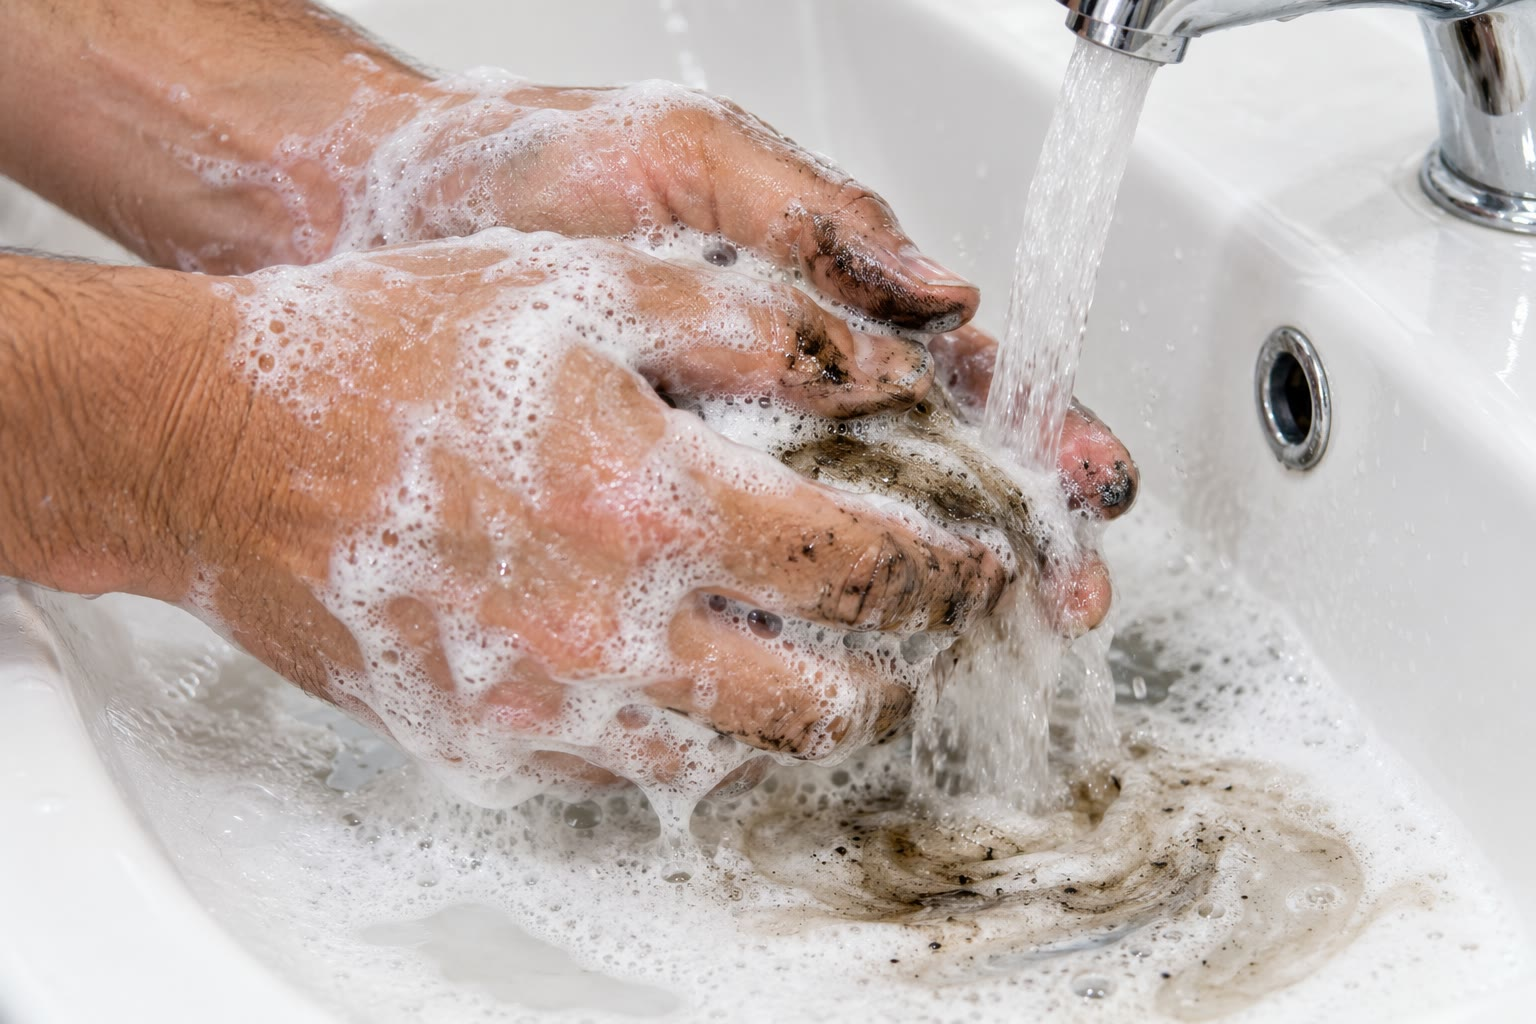
\includegraphics[width=0.48\linewidth]{images/book1/ai/g11-greasy-hands.jpg}

{\small Vette handen wassen: zeep voert het vet af in \omterm{def:g11:dissolution:amphiphilic}{micellen}.}
\end{omfigure}

\begin{remark}[Hard water en kalkzeep]\label{rem:g11:dissolution:scum}
Hard water bevat veel calciumionen \ce{Ca^{2+}} en magnesiumionen
\ce{Mg^{2+}}, opgelost uit de gesteenten waar het doorheen is gestroomd.
Met stearaationen vormen ze een \omterm{def:g9:ions:precipitate}{neerslag} (\cref{ch:g9:ions}),
calciumstearaat:
\[
  \ce{2C17H35COO- + Ca^{2+} -> Ca(C17H35COO)2(s)} .
\]
Deze grijzige vaste stof is de kalkzeep die een rand in een wastafel
vormt, en elk zeepion dat erin vastzit, is verloren voor het wassen: in
hard water schuimt zeep slecht, tot er genoeg is toegevoegd om al het
calcium neer te slaan.
\end{remark}

\begin{omfigure}
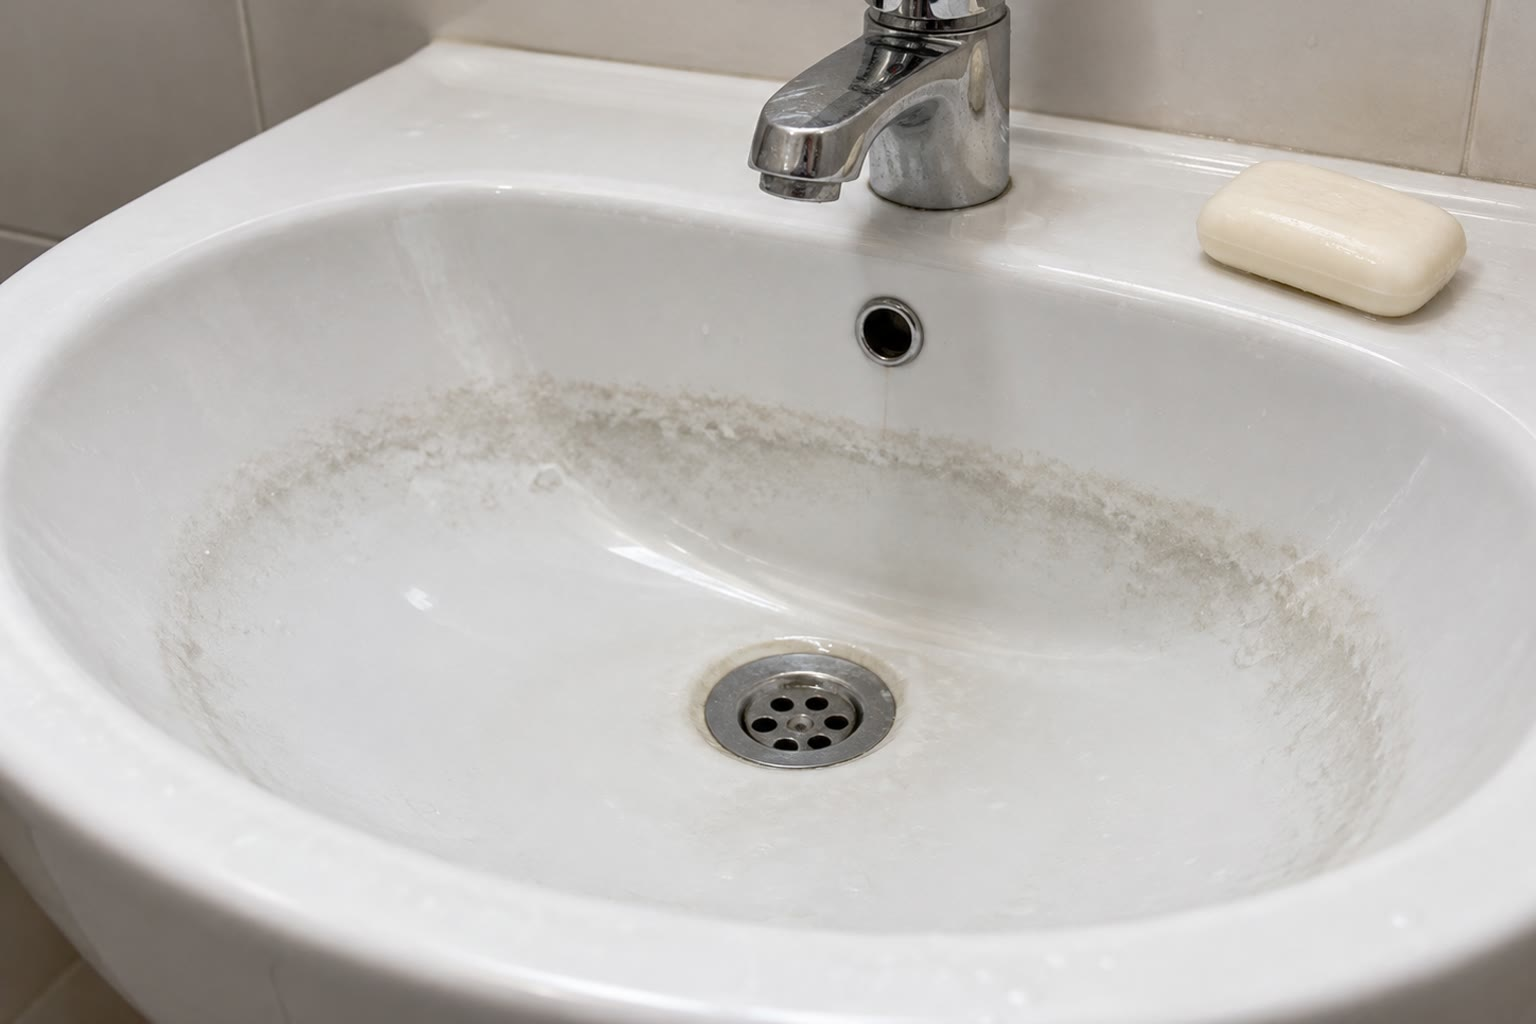
\includegraphics[width=0.45\linewidth]{images/book1/ai/g11-soap-scum.jpg}

{\small Kalkzeep in een wastafel: calciumstearaat, neergeslagen door hard
water.}
\end{omfigure}

\section{Oefeningen}


\begin{exercise}[$\star$]\label{exo:g11:dissolution:1}
Schrijf de oplosvergelijkingen in water op van natriumchloride \ce{NaCl},
calciumchloride \ce{CaCl2}, natriumsulfaat \ce{Na2SO4} en
aluminiumchloride \ce{AlCl3}.
\end{exercise}

\begin{exercise}[$\star$]\label{exo:g11:dissolution:2}
Een oplossing van natriumsulfaat heeft $c = \qty{0.050}{mol/L}$. Geef de
concentraties van de natriumionen en van de sulfaationen.
\end{exercise}

\begin{exercise}[$\star$]\label{exo:g11:dissolution:3}
Wat wordt er bedoeld met de \omterm{def:g11:dissolution:solvation}{hydratatie} van een \omterm{def:g9:ions:ion}{ion}? Welk uiteinde van een
watermolecuul wijst naar een \omterm{def:g9:ions:ion}{kation}, welk naar een \omterm{def:g9:ions:ion}{anion}? Waarom?
\end{exercise}

\begin{exercise}[$\star$]\label{exo:g11:dissolution:4}
Er wordt \qty{2.67}{g} aluminiumchloride opgelost tot \qty{200.0}{mL}
oplossing. Bereken de concentratie van de oplossing en van elk \omterm{def:g9:ions:ion}{ion}.
\end{exercise}

\begin{exercise}[$\star$]\label{exo:g11:dissolution:5}
Benoem elk deel van het stearaation als \omterm{def:g11:dissolution:hydrophilic}{hydrofiel} of \omterm{def:g11:dissolution:hydrophilic}{hydrofoob}, en zeg
waarom.
\end{exercise}

\begin{exercise}[$\star\star$]\label{exo:g11:dissolution:6}
Welk \omterm{def:g6:solutions-and-solubility:solute}{oplosmiddel}, water of cyclohexaan, zou je kiezen om op te lossen:
zout; kaarsvet (lange koolwaterstofketens); suiker (veel
\ce{O-H}-groepen); jood? Verantwoord elke keuze.
\end{exercise}

\begin{exercise}[$\star\star$]\label{exo:g11:dissolution:7}
Ethanol \ce{CH3-CH2-OH} \omterm{def:g2:mixing-and-dissolving:mix}{mengt} in alle verhoudingen met water, maar hexaan
\ce{C6H14} \omterm{def:g2:mixing-and-dissolving:mix}{mengt} niet met water. Leg uit.
\end{exercise}

\begin{exercise}[$\star\star$]\label{exo:g11:dissolution:8}
Kijk naar de figuur van de \omterm{def:g11:dissolution:amphiphilic}{micel}. Waarom zitten de staarten binnenin en de
koppen aan de buitenkant? Waarom vloeien twee \omterm{def:g11:dissolution:amphiphilic}{micellen} niet samen tot één
grotere vetdruppel?
\end{exercise}

\begin{exercise}[$\star\star$]\label{exo:g11:dissolution:9}
Een plantengeur is opgelost in water. Om hem te extraheren, kan een
scheikundige ethanol of cyclohexaan gebruiken. Welk van de twee is
geschikt, en waarom het andere niet (denk aan mengbaarheid)?
\end{exercise}

\begin{exercise}[$\star\star$]\label{exo:g11:dissolution:10}
Waarom ligt bij de joodextractie de cyclohexaanlaag bovenop? Welke laag
wordt via de kraan afgetapt? Waar zit het jood aan het eind?
\end{exercise}

\begin{exercise}[$\star\star$]\label{exo:g11:dissolution:11}
Een blauwe kopersulfaatoplossing wordt geschud met cyclohexaan. Wat
gebeurt er met de blauwe kleur? Leg uit.
\end{exercise}

\begin{exercise}[$\star\star\star$]\label{exo:g11:dissolution:12}
Hoeveel calciumchloride moet je \omterm{def:g2:mixing-and-dissolving:dissolve}{oplossen} om \qty{250.0}{mL} oplossing te
maken waarin $[\ce{Cl-}] = \qty{0.300}{mol/L}$?
\end{exercise}

\begin{exercise}[$\star\star\star$]\label{exo:g11:dissolution:13}
In een monster zeewater blijkt \qty{0.010}{mol/L} calciumionen en
\qty{0.053}{mol/L} magnesiumionen te zitten. Leg uit waarom gewone zeep in
zeewater heel slecht schuimt. Hoeveel natriumstearaat zouden alleen de
calciumionen van één liter zeewater neerslaan?
\end{exercise}

\begin{exercise}[$\star\star\star$]\label{exo:g11:dissolution:14}
Er wordt \qty{100.0}{mL} natriumchlorideoplossing met \qty{0.20}{mol/L}
gemengd met \qty{100.0}{mL} calciumchlorideoplossing met
\qty{0.10}{mol/L}. Er ontstaat geen \omterm{def:g9:ions:precipitate}{neerslag}. Bereken de concentraties
van \ce{Na+}, \ce{Ca^{2+}} en \ce{Cl-} in het \omterm{def:g6:pure-substances-and-mixtures:mixture}{mengsel}, en controleer dat
het neutraal is.
\end{exercise}

\begin{exercise}[$\star\star\star$]\label{exo:g11:dissolution:15}
% ledger: sol:I2-water, sol:I2-heptane, rho:heptane
Jood \omterm{def:g2:mixing-and-dissolving:dissolve}{lost op} tot ongeveer \qty{0.3}{g} per liter water en \qty{17}{g} per
kilogram heptaan. Heptaan heeft een dichtheid van ongeveer
\qty{0.68}{kg/L}. Hoeveel keer meer jood kan een liter heptaan bevatten
dan een liter water? Wat betekent dat voor een \omterm{def:g10:chemical-species:extraction}{extractie}?
\end{exercise}

\section{Probleem: Zeep en hard water}

\begin{problem}[{Weekendprobleem --- hoeveel zeep gaat er in een bad met
hard water verloren als kalkzeep?}]
\label{pb:g11:dissolution:1}
% ledger: aw:Ca, aw:Mg, aw:C, aw:H, aw:O, aw:Na
Een kraanwater bevat per liter \qty{120}{mg} calciumionen en \qty{24}{mg}
magnesiumionen. Een bad wordt gevuld met \qty{150}{L} ervan, en de bader
gebruikt een zeep van natriumstearaat, \ce{C17H35COONa}.

\medskip
\noindent\textbf{Deel I --- Wat er in het water zit.}
\begin{enumerate}
  \item Waar komen de calcium- en magnesiumionen van kraanwater vandaan?
  \item Bereken de \omterm{def:g10:concentration-and-dilution:molar-concentration}{molaire concentraties} van de calciumionen en van de
        magnesiumionen.
  \item De calciumionen gaan samen met waterstofcarbonaationen,
        \ce{HCO3-}, alsof er calciumwaterstofcarbonaat \ce{Ca(HCO3)2}
        was opgelost. Schrijf die oplosvergelijking op, en leid daaruit
        de concentratie waterstofcarbonaationen af die bij het calcium
        hoort.
  \item Welke hoeveelheid calciumionen bevat het bad?
\end{enumerate}

\medskip
\noindent\textbf{Deel II --- De zeep.}
\begin{enumerate}[resume]
  \item Bereken de \omterm{def:g10:the-mole:molar-mass}{molaire massa} van natriumstearaat.
  \item Schrijf de oplosvergelijking in water op.
  \item Welk deel van het stearaation is \omterm{def:g11:dissolution:hydrophilic}{hydrofiel}, welk \omterm{def:g11:dissolution:hydrophilic}{hydrofoob}? Waarom
        heet het \omterm{def:g11:dissolution:amphiphilic}{amfifiel}?
  \item Beschrijf een \omterm{def:g11:dissolution:amphiphilic}{micel}, en leg uit hoe die vet van de huid
        verwijdert.
  \item Waarom moet zeep in water opgelost worden, en niet in olie, om te
        wassen?
\end{enumerate}

\medskip
\noindent\textbf{Deel III --- Kalkzeep.}
\begin{enumerate}[resume]
  \item Schrijf de vergelijking op van de \omterm{def:g9:ions:precipitate}{neerslagreactie} van
        calciumstearaat. Controleer dat de lading klopt.
  \item Vul de \omterm{def:g10:reaction-progress-table:extent}{voortgangstabel} in voor \qty{1.00}{L} kraanwater en
        stearaationen in overmaat. Welke \omterm{def:g7:chemical-reactions:reactant}{beginstof} is beperkend?
  \item Welke hoeveelheid stearaationen gaat er per liter verloren aan
        het calcium?
  \item Bereken de \omterm{def:g10:the-mole:molar-mass}{molaire massa} van calciumstearaat, en de massa
        kalkzeep die per liter ontstaat.
  \item Magnesiumstearaat slaat op dezelfde manier neer. Welke
        hoeveelheid stearaat nemen de magnesiumionen per liter in beslag?
\end{enumerate}

\medskip
\noindent\textbf{Deel IV --- Het bad.}
\begin{enumerate}[resume]
  \item Welke hoeveelheid stearaationen slaat het calcium van het hele bad
        neer?
  \item Hoeveel zeep is dat?
  \item Hoeveel zeep gaat er in totaal verloren als je het magnesium
        meetelt?
  \item Stukken zeep wegen ongeveer \qty{100}{g}. Hoeveel stukken neemt
        het calcium alleen in beslag?
  \item Geef het eindantwoord: hoeveel zeep laat het calcium van één bad
        van \qty{150}{L} van dit water verloren gaan als kalkzeep?
\end{enumerate}
\end{problem}
